%%%%%%%%%%%%%%%%%%%%%%%%%%%%%%%%%%%%%%%%%%%%%%%%%%%%%%%%%%%%%%%%%%%%%%%%
\chapter{Object Detection}
%%%%%%%%%%%%%%%%%%%%%%%%%%%%%%%%%%%%%%%%%%%%%%%%%%%%%%%%%%%%%%%%%%%%%%%%
Object detection aims to locate objects in a given image and assign them to their \bld{class} (also called category or label). For illustration see Figure \ref{fig:od}. Generally, the task can be broken down into three steps: \bld{informative region selection}, \bld{feature extraction}, and \bld{classification}. In the first step, the method has to determine regions to which we apply the feature extraction. The feature extractor outputs a semantic numerical representation for each selected region is then used to predict the target's class. Note that, these steps are not fixed and the pipeline can vary.

\begin{figure}[h]
    \centering
    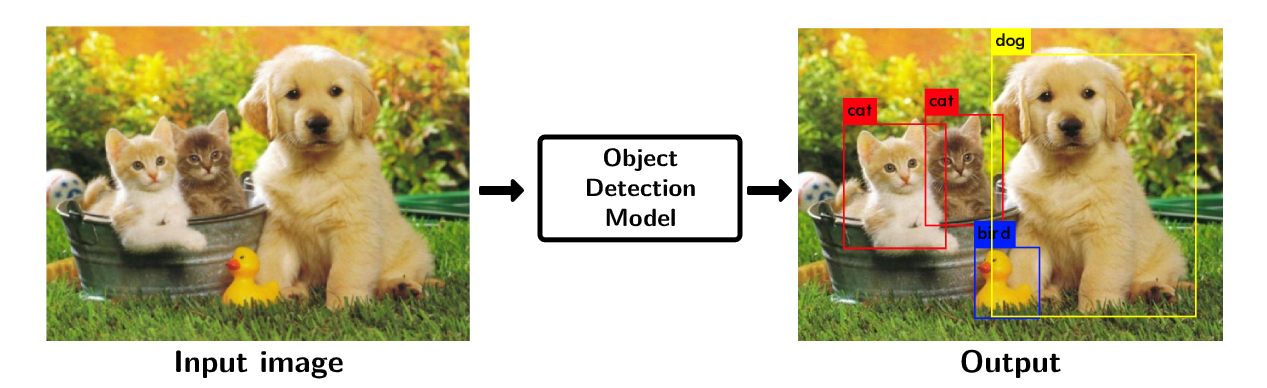
\includegraphics[width=0.9\linewidth]{Sources/Figures/objectdetection.png}
    \caption{A high-level illustration of an object detection pipeline. Adapted from \cite{objectdetectionfigure}.}
    \label{fig:od}
\end{figure}

Traditionally, engineers had to hand-craft feature extractors using algorithms such as SIFT \cite{sift}, SURF \cite{surf}, or HOG \cite{hog}. These methods are combined with well-established classification algorithms such as Support Vector Machines (SVM) \cite{svm}. Since this approach needs manual designing, it can be very demanding.

Deep learning methods introduced an end-to-end learning approach, which means that the model only takes a given set of annotated images to learn to detect key features, localize the objects, and classify them. So the hard work is done mainly by the model itself. This approach outperforms the traditional pipelines by a significant margin with respect to illumination and viewpoint changes \cite{outperforming}. We describe deep learning in detail in the Chapter \ref{deep_learning_chapter}. But firstly, let us describe how to measure the performance of object detectors.

% \begin{figure}[h]
%     \centering
%     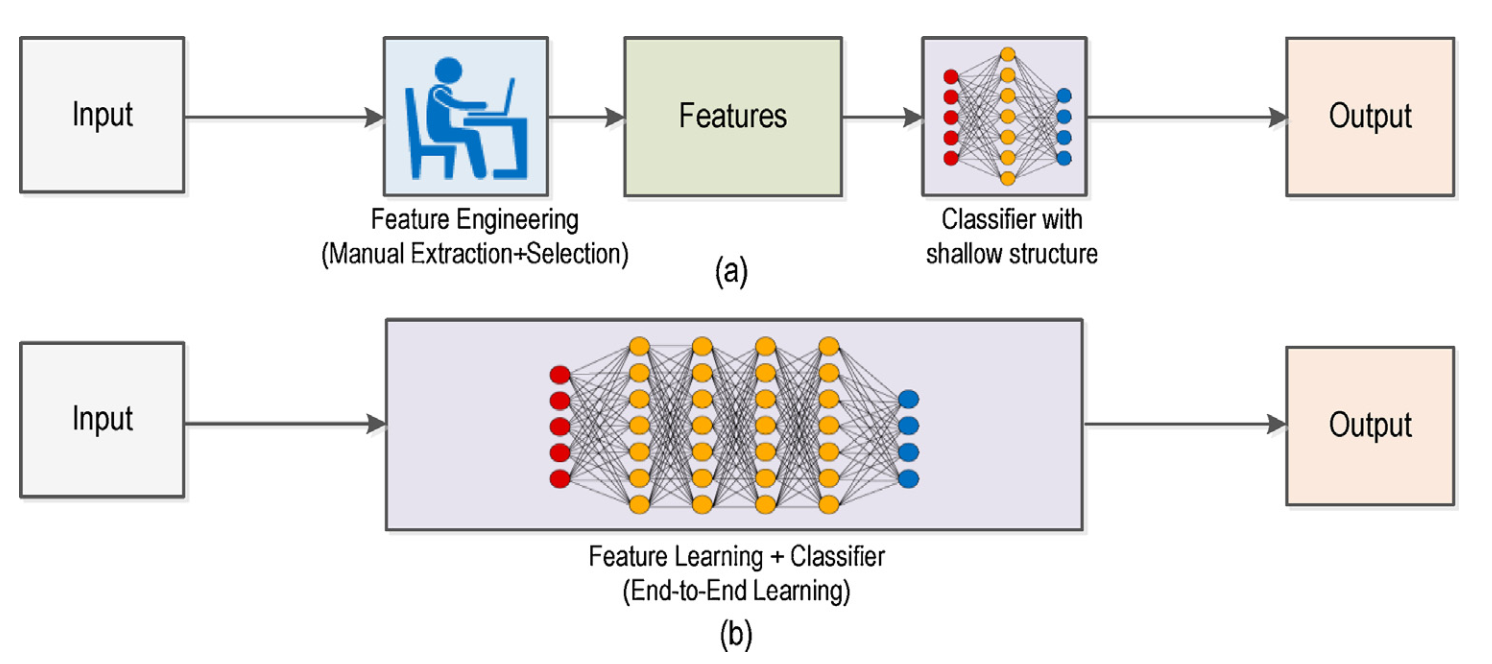
\includegraphics[width=\linewidth]{Sources/Figures/comparison.png}
%     \caption{Comparison of: (a) Traditional approach and (b) Deep learning approach. Adapted from \cite{comparison_illustration}. \todo{Zmenit obrazek, clovek mate.}}
%     \label{fig:comparison}
% \end{figure}

\section{Evaluation Metrics}
Firstly, let us define evaluation metrics for binary classification. Consider two classes we want to predict: \bld{positive (P)} and \bld{negative (N)}. Let
\begin{itemize}
    \item \bld{true positives (TP)} be correctly predicted P cases,
    \item \bld{true negatives (TN)} be correctly predicted N cases,
    \item \bld{false negatives (FN)} be all P cases we wrongly predicted as N,
    \item \bld{false positives (FP)} be all N cases we wrongly predicted as P.
\end{itemize}
Suppose we want to focus on the performance of P cases prediction. We define metrics \bld{precision} and \bld{recall} as follows:
$$
    \text{precision} = \frac{\text{TP}}{\text{TP} + \text{FP}}, \\
    \text{recall} = \frac{\text{TP}}{\text{TP} + \text{FN}}.
$$
Precision is also known as a positive predictive value, i.e., how many of the positive predictions (TP + FP) actually belong to P class. Recall is known as a true positive rate and it measures how many TP we have predicted out of all actual P cases (TP + FN). There is a trade-off relationship between these metrics. If we increase the precision (e.g., by setting more strict constraints for assigning TP to a prediction), the recall decreases as there would be more FN cases, and vice versa. 

For an object detection model evaluation, we can suppose that TP represents correctly detected object. Similarly, FP can be viewed as a wrongly detected object or duplicate detection. We would like to combine the precision and recall to a single composite score -- \bld{mean average precision (mAP)}. However, before we delve into its definition, let us first describe how to determine the TP and FP from the model's predictions.

Models output a list of predictions that are defined by \bld{bounding box} coordinates (the boundaries of the detected object), \bld{predicted class}, and \bld{confidence score} of the prediction. To determine if the detection is correct, we need to define \bld{Intersection-over-Union (IoU)}. IoU is defined as a proportion of the area of intersection (overlap between predicted bounding box and the ground-truth bounding box) and the area of union (see Figure \ref{fig:iou}):
$$
    \text{IoU} = \frac{\text{area of intersection}}{\text{area of union}}.
$$

\begin{figure}[h]
    \centering
    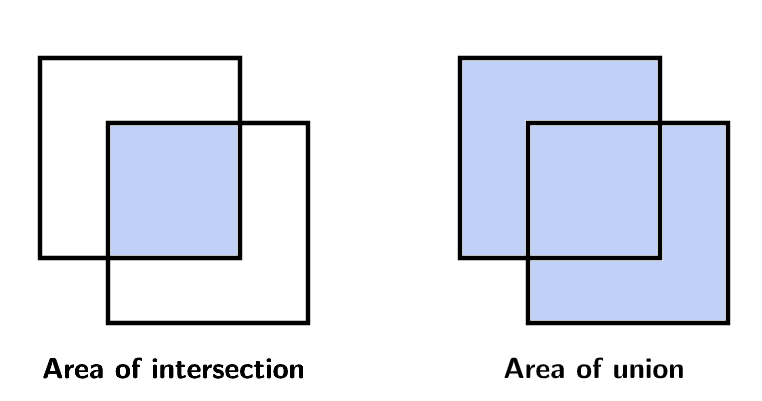
\includegraphics[width=0.6\linewidth]{Sources/Figures/iou.png}
    \caption{Illustration of two bounding boxes and the two types of areas they form.}
    \label{fig:iou}
\end{figure}
We simply declare the prediction as a TP if the IoU of the ground-truth bounding box and the predicted bounding box is greater than a fixed IoU threshold. Otherwise the prediction is considered as a FP. Now that we know how to determine the TP and FP cases, we can define mAP.

Mean average precision is an averaged \bld{average precision (AP)} over all classes. Let us define AP for some class $c$. We denote it as AP$_{c}$. For illustration, consider a simplified example: we collect all predictions for the class $c$ from all test images, and we rank them by the confidence score. Let \bld{positive predictions} be those predictions that have IoU > 0.5. If there are more positive predictions for a single object, only the prediction with a higher confidence score is considered to be a TP. See the example Table \ref{tab:ap}. In the definition of AP, precision is defined as the proportion of all predictions above the rank which are TP. Whereas recall is defined as the proportion of TP ranked above a given rank and all positive predictions.
\begin{table}[H]
\centering 
\begin{threeparttable}
\begin{tabular}{|c|c|c|c|c|c|}
\hline
\bld{rank} & \bld{IoU > 0.5} & \bld{confidence score} & \bld{TP/FP} & \bld{Precision} & \bld{Recall} \\
\hline
1 & yes & 98 \% & TP     & 1.00  & 0.2  \\
2 & yes & 88 \% & FP$^*$  & 0.50  & 0.2 \\
3 & yes & 78 \% & TP     & 0.67  & 0.4  \\
4 & yes & 75 \% & TP     & 0.75  & 0.6  \\
5 & no  & 60 \% & FP     & 0.60  & 0.6  \\
6 & yes & 59 \% & TP     & 0.67  & 0.8  \\
\hline
\end{tabular}
\begin{tablenotes}
      \small
      \item  $^*$ consider this example as a duplicate of the rank 1 example.
\end{tablenotes}
\caption{An example of predictions.}
\label{tab:ap}
\end{threeparttable}
\end{table}

Let us explain the calculation behind the third row. The precision is $2/3 \doteq 0.67$, because there are 2 TP out of 3 predictions above the third row (including the row). The recall is $2/5 = 0.4$, since there are 2 TP out of 5 positive predictions (IoU > 0.5). As we can see, the precision has a "zigzag" pattern as we go down the ranking. Whereas the recall is increasing. 

The AP$_c$ is defined as an \bld{area under the precision-recall curve} (see Figure \ref{fig:precisionrecall}). To reduce the impact of the zigzags, we interpolate the curve at each recall value $r$ by taking the maximum precision $p_\text{interp}$ measured "to the right":
$$
p_\text{interp}(r) = \max\limits_{\hat{r}:\hat{r} \geq r} p(\hat{r}),
$$
where $p(\hat{r})$ is the measured precision at the measured recall $\hat{r}$. We obtain a monotonically decreasing curve that can be numerically integrated as it is a piecewise constant (see the red dashed curve in Figure \ref{fig:precisionrecall}). We sample all unique recall values $R$ and compute AP$_c$ as a sum of rectangular blocks as follows:
$$
\text{AP}_c = \sum\limits^{\lvert R\rvert - 1}_{n = 0} (r_{n+1} - r_n) \cdot p_\text{interp}(r_{n+1}).
$$

\begin{figure}[H]
    \centering
    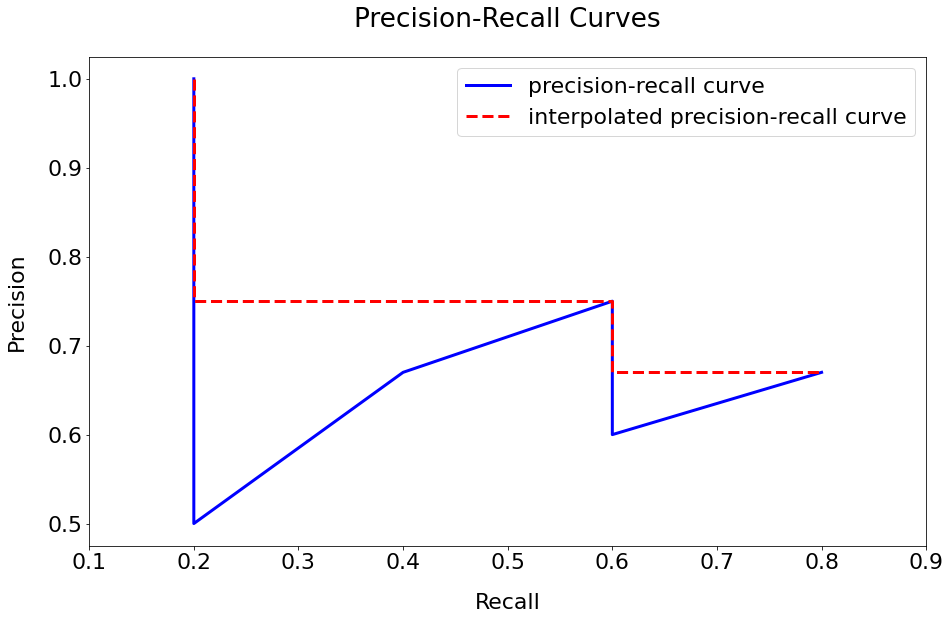
\includegraphics[width=0.8\linewidth]{Sources/Figures/precisionrecall.png}
    \caption{Precision-recall curves.}
    \label{fig:precisionrecall}
\end{figure}

We then get the final mAP by averaging all AP$_c$ for every class (let $C$ be the set of all classes):
$$
    \text{mAP} = \frac{1}{\lvert C \rvert} \cdot \sum_{ c\in C} \text{AP}_c.
$$
The VOC competitions \cite{voc} used this metric for a fixed IoU = 0.5 threshold. However, for our evaluation, we use the \bld{updated COCO challenge metric} \cite{coco} that averages the mAP over 10~different IoU thresholds (from 0.50 to 0.95 with 0.05 step size). We denote it as AP$_{.50:.05:.90}$ = AP. Similarly, for single IoU thresholds we have AP$_{50}$ (the standard VOC metric) and AP$_{75}$ (a~strict metric). They also define AP$_\text{small}$, AP$_\text{medium}$, and AP$_\text{large}$ for varying object's size:
\begin{itemize}
    \item AP$_\text{small}$ is an AP for small objects (bounding box area < $32^2$ px),
    \item AP$_\text{medium}$ is an AP for medium objects ($32^2$ < area < $96^2$ px),
    \item AP$_\text{large}$ is an AP for large objects (area > $96^2$ px).
\end{itemize}
Note that they do not make distinction between mAP and AP. Henceforth, whenever we refer to the AP, we mean the primary COCO metric AP$_{.50:.05:.90}$. 










